\documentclass[11pt]{article}

% ---------------------------------------------------------------
% Post-Monetary Political Economy & Local-First Software Monograph
% Compiles cleanly with Tectonic / XeLaTeX / pdfLaTeX + BibTeX.
% Target repositories/venues: Zenodo, SSRN, PhilArchive,
% Journal of Institutional Economics, New Political Economy, Big Data & Society.
% ---------------------------------------------------------------
\usepackage[T1]{fontenc}
\usepackage[utf8]{inputenc}
\usepackage{lmodern}
\usepackage{microtype}
\usepackage[margin=1.00in]{geometry}
\usepackage{amsmath,amssymb}
\usepackage{booktabs}
\usepackage{tabularx}
\usepackage{array}
\usepackage{enumitem}
\usepackage[section]{placeins}
\usepackage[authoryear,round]{natbib}
\usepackage{xcolor}
\usepackage{tikz}
\usetikzlibrary{arrows.meta,positioning,fit,backgrounds,calc}
\PassOptionsToPackage{hyphens}{url}
\usepackage[hidelinks]{hyperref}
\usepackage{xurl}

\newcolumntype{Y}{>{\raggedright\hskip0pt\emergencystretch=1.5em\arraybackslash}X}
\newcolumntype{P}[1]{>{\raggedright\hskip0pt\emergencystretch=1.5em\arraybackslash}p{#1}}
\renewcommand{\arraystretch}{1.18}
\tolerance=1200
\setlength{\emergencystretch}{3em}
\hfuzz=0.5pt
\Urlmuskip=0mu plus 2mu\relax
\expandafter\def\expandafter\UrlBreaks\expandafter{\UrlBreaks\do\-\do\_}
\setlist{itemsep=3pt,topsep=4pt}

\definecolor{forest}{HTML}{0B3F30}
\definecolor{sienna}{HTML}{8B3A1B}
\definecolor{slate}{HTML}{2B6CB0}
\definecolor{sand}{HTML}{F4EBDD}

\title{\textbf{From Money-as-Veto to Memory-as-Protocol}\\[4pt]
\large Local Open-Source Software, Polycentric Demand Coordination, and Trust-Based Clearing}

\author{\textbf{Dima Baker}\\
Collective Intelligence Network\\
{\small\texttt{https://cintnet.org} $\cdot$ Companion Technical Archive: \texttt{doi:10.5281/zenodo.24560618}}}

\date{November 2026}

\begin{document}
\maketitle

% ===============================================================
\begin{abstract}
Orthodox economics treats money as a neutral veil over barter, while contemporary software markets treat software as a rented cloud service. Building on Mason and Jayadev's \emph{Against Money} (2026), Keynes's monetary theory of production, and Kocherlakota's formal theorem that \emph{money is memory} (1998), we argue that legacy monetary institutions and proprietary Software-as-a-Service (SaaS) enact twin artificial scarcities: financial balance sheets exercise an oligopolistic veto over real cooperation, while cloud platforms impose rent-extracting tollbooths over non-rivalrous mathematical instructions. Yet critiques of money historically stalled because critics offered no decentralized mechanism capable of replacing price signals without reverting to blind central planning. We resolve this impasse by articulating a three-layer post-monetary architecture grounded in the Collective Intelligence Network (CIN): (1)~\emph{local-first, open-source personal software} running strictly on user hardware as a polycentric demand-coordination layer; (2)~\emph{thin, open-source federated protocols} carrying cryptographically attested institutional memory governed by risk-scaled asymmetric transparency; and (3)~\emph{physical-unit multilateral clearing} paired with bounded zero-interest mutual credit and cooperative productive equity. Throughout, we confront four sharp failure modes---social-credit panopticon drift, hard physical rivalry, open-source maintenance exhaustion alongside shared-state network physics, and institutional transition---demonstrating how progressive dual-layer expansion unbundles money's veto power without sacrificing privacy, scarcity discipline, or decentralized local knowledge.
\end{abstract}

\noindent\textbf{Keywords:} post-monetary economics, money is memory, local-first software, open-source commons, polycentric demand coordination, mutual credit, asymmetric transparency, institutional trust.

% ===============================================================
\section{Introduction: The Twin Artificial Scarcities}\label{sec:intro}

Two background myths quietly govern the modern digital economy. The first is the \textbf{barter myth of money}: the textbook story that human societies began by trading fish for grain on desert islands, invented coins purely as a frictionless convenience, and now rely on prices as a neutral mirror of physical reality. The second is the \textbf{service myth of software}: the commercial assumption that computational tools naturally exist as centralized, subscription-gated cloud platforms operated by corporate intermediaries who hold custody of user data, workflows, and social graphs.

Both myths collapse under historical and technical scrutiny. As economic historians, anthropologists, and monetary theorists have documented for over a century, no pure barter economy has ever existed \citep{innes1913money, humphrey1985barter, graeber2011debt}. Following John Maynard \citet{keynes1933monetary, keynes1936general}, \citet{mason2026against} demonstrate in \emph{Against Money} that money is never a neutral veil over an already-settled ``real economy.'' Production runs in reverse of the textbook fable: what gets built depends on what gets financed. Private credit hierarchies already operate as centralized economic planning by a handful of financial balance sheets---steering hundreds of billions of dollars toward speculative computing clusters while decarbonization, preventive medicine, and resilient civic infrastructure struggle for credit \citep{mason2014fisher, jayadev2018mmt, mason2026against}. In this light, capital acts less as a physical stock of helpful tools and more as a \textbf{veto over cooperation}: idle factories, exclusionary patents, and liquidity freezes prevent willing producers and households from coordinating even when real materials, skills, and needs stand side by side.

Simultaneously, \textbf{Software-as-a-Service (SaaS)} represents the purest digital incarnation of that veto. Mathematically, software is non-rivalrous: once written, copying an instruction set across ten million local machines carries near-zero marginal physical cost \citep{benkler2002coase}. Turning non-rivalrous code into a recurring service requires artificially relocating execution and state onto remote corporate servers, erecting proprietary API walls, and converting ordinary digital tools into behavioral tollbooths \citep{kleppmann2019local, zuboff2019surveillance, balkin2016fiduciaries}. As frontier artificial intelligence compresses the marginal cost of authoring and adapting software toward zero, the economic justification for renting everyday software as a hosted service evaporates entirely.

Crucially, as \citet{mason2026against} emphasize, national income metrics such as ``real GDP'' systematically conceal how much of modern civilization \emph{already} functions outside monetary exchange: open-source operating systems and libraries, Wikipedia, basic scientific research, public education, public health, household care, and even the internal non-market logistics inside large private corporations \citep{coase1937firm, benkler2002coase}. Yet heterodox critiques of money have historically stopped short of specifying the concrete computational and institutional protocols needed to coordinate complex, dispersed human demand without recreating a brittle central-planning bureaucracy.

This paper supplies that missing systems architecture. Building on the formal engineering stack and empirical benchmarks of the Collective Intelligence Network (CIN) \citep{baker2026cin}, we unite three insights:
\begin{enumerate}
  \item \textbf{Money is a lossy proxy for social memory} \citep{kocherlakota1998memory}---a low-bandwidth compression artifact that modern cryptographic provenance and federated logs can now outperform without financial gatekeeping.
  \item \textbf{Software's natural state is local and open source} \citep{kleppmann2019local, benkler2002coase}---running strictly on the user's hardware for execution and state, connected only through thin, open, neutral protocols where multi-party coordination is physically irreducible.
  \item \textbf{Demand coordination and exchange can be unbundled into verifiable institutional trust and multilateral clearing}---replacing speculative financial veto power with structured demand intents, physical-unit cycle netting, zero-interest mutual credit, and risk-scaled asymmetric transparency.
\end{enumerate}

Figure~\ref{fig:unbundling} summarizes this architectural shift from monolithic monetary and cloud-SaaS vetoes to a three-layer local-first demand and trust-clearing stack.

\begin{figure}[ht]
\centering
\resizebox{\textwidth}{!}{%
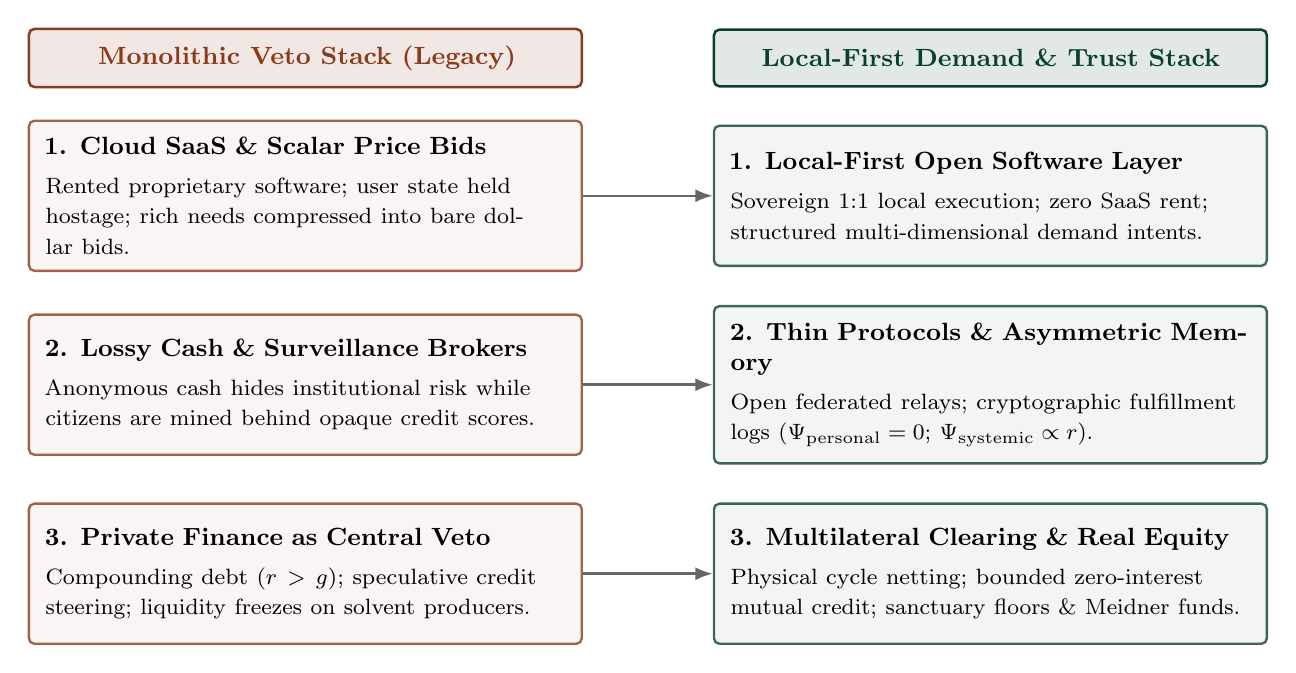
\begin{tikzpicture}[
  font=\small,
  box/.style={draw, rounded corners=2pt, text width=6.6cm, minimum height=1.78cm, align=left, inner sep=6pt, line width=0.85pt},
  hdr/.style={draw, rounded corners=2pt, text width=6.6cm, minimum height=0.72cm, align=center, font=\small\bfseries, inner sep=6pt, line width=0.9pt},
  arr/.style={-{Latex[length=2.2mm]}, black!60, line width=0.9pt}
]
% Headers
\node[hdr, draw=sienna, fill=sienna!12, text=sienna] (hl) at (-4.35, 6.95) {Monolithic Veto Stack (Legacy)};
\node[hdr, draw=forest, fill=forest!12, text=forest] (hr) at (4.35, 6.95) {Local-First Demand \& Trust Stack};

% Layer 1: Software & Demand
\node[box, draw=sienna!80, fill=sienna!5] (l1) at (-4.35, 5.20) {\textbf{1. Cloud SaaS \& Scalar Price Bids}\\[3pt]{\footnotesize Rented proprietary software; user state held hostage; rich needs compressed into bare dollar bids.}};
\node[box, draw=forest!80, fill=forest!5] (r1) at (4.35, 5.20) {\textbf{1. Local-First Open Software Layer}\\[3pt]{\footnotesize Sovereign 1:1 local execution; zero SaaS rent; structured multi-dimensional demand intents.}};

% Layer 2: Memory & Trust
\node[box, draw=sienna!80, fill=sienna!5] (l2) at (-4.35, 2.80) {\textbf{2. Lossy Cash \& Surveillance Brokers}\\[3pt]{\footnotesize Anonymous cash hides institutional risk while citizens are mined behind opaque credit scores.}};
\node[box, draw=forest!80, fill=forest!5] (r2) at (4.35, 2.80) {\textbf{2. Thin Protocols \& Asymmetric Memory}\\[3pt]{\footnotesize Open federated relays; cryptographic fulfillment logs ($\Psi_{\mathrm{personal}}=0$; $\Psi_{\mathrm{systemic}} \propto r$).}};

% Layer 3: Clearing & Capital
\node[box, draw=sienna!80, fill=sienna!5] (l3) at (-4.35, 0.40) {\textbf{3. Private Finance as Central Veto}\\[3pt]{\footnotesize Compounding debt ($r>g$); speculative credit steering; liquidity freezes on solvent producers.}};
\node[box, draw=forest!80, fill=forest!5] (r3) at (4.35, 0.40) {\textbf{3. Multilateral Clearing \& Real Equity}\\[3pt]{\footnotesize Physical cycle netting; bounded zero-interest mutual credit; sanctuary floors \& Meidner funds.}};

\draw[arr] (l1.east) -- (r1.west);
\draw[arr] (l2.east) -- (r2.west);
\draw[arr] (l3.east) -- (r3.west);
\end{tikzpicture}%
}
\caption{Unbundling the twin artificial scarcities of legacy monetary vetoes and proprietary Cloud SaaS into a three-layer architecture of local-first open-source software, asymmetric institutional memory, and multilateral real-economy clearing.}
\label{fig:unbundling}
\end{figure}

% ===============================================================
\section{Unbundling Money: From Lossy Scalar Cash to Cryptographic Memory}\label{sec:memory}

\subsection{Kocherlakota's Theorem and the Compression Cost of Prices}

To move beyond money responsibly, one must first state clearly what useful computational function money actually performed. In a landmark theorem in monetary economics, \citet{kocherlakota1998memory} proved that \textbf{money is mathematically equivalent to a primitive form of memory}. In dynamic decentralized economies where strangers interact sequentially, cooperation breaks down without a record of whether an agent previously contributed to others. When societies lack reliable, low-cost collective memory of past actions, an unforgeable physical or ledger token acts as a crude proxy: holding cash signals, in one compressed scalar number, that someone previously delivered accepted output (or held financial privilege). Kocherlakota proved that if an economy possesses a reliable historical memory of relevant commitments and fulfillments, \emph{any allocation achievable with money is achievable without it}---and strictly richer conditional allocations become feasible.

Viewing Kocherlakota's result alongside \citet{mason2026against} exposes why legacy money fails simultaneously as an \emph{informational} tool and a \emph{social} institution:
\begin{equation}
  \Pi_{\mathrm{price}} : \mathcal{X}_{\mathrm{need}} \longrightarrow \mathbb{R}_{>0}, \qquad \text{whereas} \qquad \mathcal{D}_{\mathrm{intent}} \times \mathcal{M}_{t}^{\mathrm{inst}} \longrightarrow \mathcal{A}_{\mathrm{clear}}.
  \label{eq:projection}
\end{equation}
A scalar price projection $\Pi_{\mathrm{price}}$ collapses deeply multi-dimensional physical and social realities---delivery urgency, geographic locality, ecological footprint, accessibility, maintenance durability, and institutional trustworthiness---into a single undifferentiated dollar figure weighted strictly by preexisting wealth. A billionaire bidding for speculative computing hardware outbids a rural clinic requesting reliable backup power not because the informational signal is superior, but because scalar currency entangles \emph{information about need} with \emph{unbounded private veto power}.

By contrast, an open cryptographic memory protocol $\mathcal{M}_{t}^{\mathrm{inst}}$ records verifiable institutional commitments, physical delivery receipts, safety audits, and clearing reciprocity across the network without collapsing them into a speculative hoarding asset. Money's useful memory function is preserved and upgraded in resolution, while its capacity to compound into an exclusionary veto is stripped away.

\subsection{Resolving the Calculation Debate Without Central Command}

Why did earlier proposals to transcend monetary exchange stall? In the classic Socialist Calculation Debate, \citet{mises1920calculation} and \citet{hayek1945knowledge} mounted a formidable epistemic critique against Otto \citet{neurath2004economic}'s wartime proposal for non-monetary \emph{calculation in kind} (\emph{Naturalrechnung}). Hayek observed that the knowledge required to coordinate an economy---which neighborhood bakery has surplus oven capacity at 4~a.m., which machinist can adapt a replacement valve, which family needs quiet evening eldercare---is tacit, dispersed, and continuously changing. No centralized planning board can aggregate that tacit knowledge into top-down production directives without fatal latency and distortion.

Later cybernetic and digital-planning projects attempted to bridge this gap. Stafford Beer's 1971--1973 \emph{Project Cybersyn} in Chile pioneered real-time industrial telemetry and Viable System recursion \citep{medina2011cybernetic}, while \citet{saros2014information} proposed a centralized digital ``General Catalogue'' through which households register consumption preferences directly with worker councils. Yet both architectures remained structurally vulnerable to central-registry bottlenecks, single-point state coercion, and rigid, low-nuance product taxonomies.

Polycentric personal software changes the geometry of Hayek's knowledge problem entirely:
\begin{itemize}
  \item \textbf{Tacit knowledge stays local.} A biological principal's lived context, routines, health needs, and aesthetic preferences remain encrypted inside a local personal memory vault governed by a 1:1 local cognitive model \citep{baker2026cin}. No central planner or cloud broker ever ingests that intimate state.
  \item \textbf{Structured demand travels peer-to-peer.} Rather than waiting for a ministry quota or submitting an impoverished cash bid, local open-source software translates lived needs into explicit, constraint-rich demand intents $d_i \in \mathcal{D}$ (quantity, timing window, local delivery bounds, repairability, verified labor/ecological provenance) broadcast selectively to regional cooperatives, producers, and federated clearing meshes.
  \item \textbf{Polycentric adaptation replaces central command.} Following Elinor \citet{ostrom1990governing, ostrom2010beyond}, nested local and regional clearing nodes reconcile matching supply and demand autonomously at the lowest feasible scale, escalating only cross-regional physical bottlenecks.
\end{itemize}

This architecture answers Hayek and Mason--Jayadev simultaneously: it preserves decentralized local knowledge without surrendering social coordination to the centralized private planning of Wall Street credit desks.

% ===============================================================
\section{The Ontology of Local-First, Non-Service Software}\label{sec:software}

\subsection{Why Software's Natural Existence Is Local and Open Source}

In \emph{Coase's Penguin}, \citet{benkler2002coase} demonstrated that open-source software (such as Linux) thrives outside both market price signals and corporate hierarchies because information goods are non-rivalrous and modular peer verification outperforms managerial command. Nearly two decades later, \citet{kleppmann2019local} formalized \emph{local-first software}: applications built on Conflict-free Replicated Data Types (CRDTs) and local storage so that users experience zero network latency, full offline operation, end-to-end encryption, and ``the Long Now'' guarantee that their data and tools outlive any vendor.

Yet the commercial web evolved in the opposite direction. Cloud SaaS normalized a deeply unnatural ontological premise: that to write a document, coordinate a neighborhood cooperative, schedule medical care, or run a business ledger, one must continuously rent execution from a remote corporation's servers. Under SaaS, software ceases to be a tool owned by its user and becomes a \textbf{service relationship mediated by permanent rent and revocable permission}. When combined with cloud-hosted AI models, this architecture transforms every daily task into metered cognitive dependency.

When AI drives the marginal cost of generating, auditing, and tailoring bespoke interfaces toward zero, the case for proprietary SaaS collapses completely. Software returns to its natural state:
\begin{enumerate}
  \item \textbf{Strictly local execution and custody:} Application binaries, adapted personal weights, and episodic state live on user-controlled hardware. No vendor can alter pricing, deprecate features, mine private drafts, or revoke access remotely.
  \item \textbf{Open source and malleable by default:} Every protocol parser, demand-matching agent, and clearing client is inspectable, forkable, and locally adaptable so users and communities can reshape tools around local workflows rather than conforming to corporate templates.
  \item \textbf{Capability-bounded external action:} When local software interacts with external networks, it acts strictly under short-lived, revocable Object-Capability leases \citep{dennis1966programming} with deterministic expiration clocks---never standing third-party credentials.
\end{enumerate}

\subsection{Two Honest Architectural Boundaries: Network Physics and Maintenance Commons}

An intellectually serious case for local open-source software must confront two realities where naive slogans (``100\% local, zero infrastructure, free labor'') break down immediately.

\paragraph{Boundary 1: Local Execution by Default, Thin Neutral Protocols for Shared State.}
While application execution, personal memory, and decision tooling belong strictly on local hardware, certain multi-party coordination primitives obey irreducible distributed-systems physics. Asynchronous message delivery when a peer's device is offline, discovery of closed multilateral trade cycles across dozens of regional firms, and tamper-evident transparency logs (IETF SCITT) require shared network relays and verifiable append-only mirrors. The architectural principle is therefore \textbf{local execution by default; thin, open-source, neutral protocols---never proprietary platforms---for shared state}. Like TCP/IP or DNS roots governed by federated cooperatives and public utilities, clearing relays carry zero proprietary application lock-in, zero behavioral monetization, and full cryptographic verifiability so any community can mirror or exit a misbehaving node without losing its local software or history.

\paragraph{Boundary 2: Sustaining Invisible Open-Source Maintenance Without SaaS Rent.}
If software ceases to be sold as a rent-bearing SaaS product, who sustains the unglamorous, high-skill labor of kernel security patching, cryptographic verification, dependency auditing, and hardware-driver upkeep? As \citet{eghbal2020working} documented in \emph{Working in Public}, modern open-source bottlenecks stem not from writing initial code, but from maintainer burnout under asymmetric user demand. Empirical studies confirm that tracking raw code output misses the ``invisible labor'' of triage, review, and care work that keeps shared digital infrastructure alive \citep{meluso2024invisible}---a strain intensified when generative AI floods repositories with cheap synthetic pull requests.

Eliminating SaaS tolls therefore requires explicit \textbf{stewardship funding decoupled from usage rent}:
\begin{itemize}
  \item \textbf{Public digital-infrastructure endowments and Meidner cooperative funds:} Regional cooperatives, municipalities, and automated productive plants fund core open-source protocol maintenance as shared civic infrastructure (analogous to bridges, water mains, and open scientific standards) \citep{meidner1978funds}.
  \item \textbf{Non-monetary verified maintenance attribution:} Cryptographically attested review, security auditing, and upkeep records accumulate non-transferable governance stewardship weight in protocol evolution---decoupling influence from capital ownership while avoiding turning care work into speculative tokens \citep{deci1999rewards}.
\end{itemize}

% ===============================================================
\section{The Polycentric Demand Layer and Asymmetric Trust Clearing}\label{sec:clearing}

\subsection{Unbundling Money's Three Tangled Functions}

Standard fiat currencies collapse three incompatible institutional functions into a single instrument: a \emph{store of compounding power}, a \emph{medium of everyday exchange}, and an \emph{accounting memory of obligations}. The CIN post-monetary architecture separates these functions cleanly across distinct, non-extractive primitives:
\begin{enumerate}
  \item \textbf{Retiring Money-as-Veto (Sanctuary Floors and Cooperative Equity):} Basic human survival---housing security, healthcare, nutrition, education, and local compute access---is anchored in unconditional Universal Basic Services and zero-decay household sanctuary floors. Long-horizon physical infrastructure is financed via \citet{meidner1978funds} cooperative capital funds fed by automated productive surpluses, removing private financial balance sheets' veto over essential real-economy investment \citep{polanyi1944great, mason2026against}.
  \item \textbf{Replacing Rent-Bearing Liquidity (Multilateral Clearing and Zero-Interest Mutual Credit):} For active inter-firm and cooperative production, local demand software routes real supply commitments into \textbf{multilateral cycle netting} \citep{fleischman2026cycles}, canceling closed obligation loops directly in physical and clearing units without touching commercial bank debt. Acyclic working-capital gaps clear through turnover-bounded, zero-interest mutual credit meshes ($\sum_{i} b_i = 0$) modeled on Switzerland's WIR Bank \citep{stodder2009wir} and Sardinia's Sardex \citep{iosifidis2018sardex}. To deter strategic urgency inflation \citep{hurwicz1972decentralized}, clearing enforces fraud-proof costly verification audits \citep{perezrichet2022falsification}.
  \item \textbf{Upgrading Coordination Memory (Verifiable Institutional Trust):} Rather than relying on hoarded currency to prove counterparties will perform, federated transparency logs record domain-scoped institutional fulfillment history directly across the network.
\end{enumerate}

\subsection{Measuring Trust Without Building a Social Credit Panopticon}

Replacing financial gatekeeping with ``network measurements of trust and transparency'' carries an acute political hazard: if applied symmetrically to individual human beings, universal trust scoring degenerates rapidly into an authoritarian social-credit panopticon that punishes dissent, disability, or social nonconformity.

To foreclose that failure mode mathematically and constitutionally, CIN enforces \textbf{Risk-Scaled Asymmetric Transparency} across Karl \citet{friston2013life}'s Markov blanket boundary:
\begin{equation}
  \Psi(r_{\mathrm{personal}}) = 0, \qquad \frac{d\Psi(r)}{dr} \ge 0 \quad \text{for institutional externality } r > r_0.
  \label{eq:asymmetric}
\end{equation}
Under Equation~\eqref{eq:asymmetric}, trust measurement obeys three non-negotiable invariants:
\begin{itemize}
  \item \textbf{Institutional and commitment-scoped only:} The network measures \emph{verifiable institutional fulfillment}---whether a grain mill delivered Grade-A flour on schedule, whether a medical device cooperative passed independent cross-lineage safety audits, whether a regional clearing node maintained zero-sum solvency, and how promptly a producer honored warranty recalls. It \textbf{never} assigns a global reputation score to a biological person's private speech, friendships, political views, or eligibility for unconditional sanctuary services.
  \item \textbf{Anti-Goodhart and anti-crowding-out bounds:} Because any scalar metric turned into a high-stakes target invites gaming \citep{strathern1997ratings} and extrinsic point systems erode intrinsic prosocial care \citep{deci1999rewards}, institutional memory remains \emph{multi-dimensional and domain-specific} (separate auditable ledgers for delivery reliability, safety provenance, ecological compliance, and mutual-credit clearing) rather than a single gamified star rating.
  \item \textbf{Post-transduction humility (\emph{Signed Is Not True}):} Cryptographic receipts prove chain of custody after digital logging, never infallible physical truth \citep{fu2018sensors}. Whenever physical deliveries, sensor readings, or fulfillment records are noisy or disputed, the protocol enforces \emph{system-borne uncertainty} and mandatory human contestability so institutional ambiguity never automatically penalizes ordinary citizens \citep{baker2026cin}.
\end{itemize}

\subsection{Arbitrating Hard Physical Scarcity Without Speculative Bidding}

A decisive critique of post-monetary economics must be confronted candidly: \emph{software is non-rivalrous, but copper, grid megawatts, hospital surgical suites, prime farmland, and skilled human hours are strictly rivalrous.} Eliminating SaaS rent and financial speculation does not make physical reality infinite. When aggregated structured demand for a scarce physical input $k$ exceeds available real capacity ($\sum_i d_{i,k} > C_k$), any viable economy requires a transparent, non-arbitrary rationing and expansion rule.

The polycentric software layer resolves rivalrous physical bottlenecks through three layered arbitration protocols rather than interest-bearing price wars:
\begin{enumerate}
  \item \textbf{Unconditional Priority Tiers (Lexicographic Essentiality):} Essential physiological and civic floors (emergency healthcare, municipal water/power, baseline nutrition, disability access) clear lexicographically ahead of discretionary industrial or luxury requests.
  \item \textbf{Transparent Physical Capacity Budgets and Bounded Clearing Numeraires:} For non-essential rivalrous inputs (peak grid energy, scarce fabrication slots, specialized transport), regional cooperatives publish real-time physical availability envelopes paired with bounded, non-compounding, expiring clearing credits. Unlike fiat currency, these clearing numeraires cannot earn compound interest, cannot be leveraged into speculative derivatives, and cannot purchase political governance votes.
  \item \textbf{Automated Capacity-Expansion Signals:} Persistent unmet structured demand ($\sum_i d_{i,k} - C_k > \tau_k$ across consecutive clearing epochs) feeds directly into public regional capacity dashboards, signaling Meidner cooperative capital funds and engineering guilds to invest real labor and materials into expanding bottleneck supply---turning scarcity signals into physical build-out rather than permanent rentier windfalls.
\end{enumerate}

% ===============================================================
\section{Comparative Architecture, Stress-Tests, and Dual-Layer Transition}\label{sec:comparison}

\subsection{Comparing Four Coordination Regimes}

Table~\ref{tab:regimes} contrasts the Local-First Demand and Trust Mesh against legacy fiat markets, centralized state planning, and Cloud SaaS platform monopolies across six structural dimensions. Table~\ref{tab:stresstests} summarizes the four structural stress-tests analyzed in Sections~\ref{sec:software}--\ref{sec:clearing} alongside their explicit protocol remedies.

\begin{table}[ht]
\centering
\footnotesize
\caption{Structural comparison of four economic and software coordination regimes.}
\label{tab:regimes}
\begin{tabularx}{\textwidth}{@{}P{2.25cm}P{2.85cm}P{2.75cm}P{2.75cm}Y@{}}
\toprule
Dimension & Legacy Fiat Markets & Centralized Planning & Cloud SaaS Monopolies & Local-First Trust \& Demand Mesh \\
\midrule
Coordination Signal & Scalar prices weighted by wealth ($p \in \mathbb{R}_{>0}^n$). & Top-down output quotas from central ministry. & Engagement feeds \& proprietary API tolls. & Structured local demand intents + verified institutional memory. \\
Veto / Rent Power & Private finance vetoes real production \citep{mason2026against}. & State bureaucracy exercises total command veto. & Platform landlord controls data, pricing, and access. & Zero SaaS rent; financial veto unbundled via clearing \& equity. \\
Local Knowledge & Preserved partially, but distorted by income inequality. & Severe Hayekian blindness to tacit local detail. & Extracted into remote behavioral profiles. & Tacit context stays encrypted locally; intents travel peer-to-peer. \\
Privacy vs.\ Visibility & Inverted: opaque banks, surveilled borrowers. & High state visibility over citizens; opaque apparatus. & Asymmetric corporate panopticon \citep{zuboff2019surveillance}. & Risk-scaled asymmetric ($\Psi_{\mathrm{personal}}=0$; $\Psi_{\mathrm{systemic}} \propto r$). \\
Software Ontology & Mixed; increasingly financialized SaaS. & Monolithic state-administered mainframes. & Hosted proprietary service (rent-seeking default). & Local-first open source; thin neutral protocols for shared state. \\
Rivalrous Scarcity & Allocated by highest cash bid; speculative bubbles. & Chronic shortages, queues, and black markets. & Algorithmic surge pricing and tiered lock-in. & Essential priority tiers + bounded clearing + Meidner expansion. \\
\bottomrule
\end{tabularx}
\end{table}

\begin{table}[ht]
\centering
\small
\caption{Four structural stress-tests of post-monetary local software systems and their protocol remedies.}
\label{tab:stresstests}
\begin{tabularx}{\textwidth}{@{}P{2.85cm}P{4.15cm}Y@{}}
\toprule
Stress-Test & Failure Mode if Unaddressed & Architectural Protocol Remedy \\
\midrule
Social Credit Panopticon & Universal trust metrics police personal speech, health, and dissent. & Enforce $\Psi(r_{\mathrm{personal}})=0$; scope trust strictly to institutional delivery, safety, and solvency; keep UBS unconditional. \\
Hard Physical Rivalry & Treating energy, copper, or clinic beds as infinite collapses supply. & Distinguish non-rivalrous code from rivalrous matter; use priority tiers, bounded non-compounding clearing credits, and capacity expansion. \\
Shared State \& Maintenance & Local-only dogma breaks async clearing; removing SaaS starves maintainers. & Local execution by default + thin open protocols for shared state; fund upkeep via digital-commons endowments and Meidner equity. \\
Transition Fragility & Overnight currency abolition triggers supply shock and breakdown. & Progressive dual-layer displacement expanding alongside legacy fiat via B2B clearing, public procurement, and cooperative capital. \\
\bottomrule
\end{tabularx}
\end{table}

\subsection{Progressive Dual-Layer Transition: Displacing the Veto Without Shock}

A sober reading of \citet{mason2026against} and \citet{polanyi1944great} cautions against utopian overnight abolition of legacy currency. Modern supply chains exhibit deeply embedded bounded rationality and legacy contractual dependencies; attempting to decree cash away overnight would produce immediate logistical collapse. Fortunately, the architecture developed here requires no central decree. Just as Linux, Wikipedia, open scientific standards, and regional mutual-credit networks already operate beside commercial markets, the local-first demand and trust mesh grows through \textbf{progressive dual-layer expansion}:
\begin{enumerate}
  \item \textbf{Phase I --- Local Open Software and Regional B2B Netting:} Households and small firms adopt local-first, open-source personal tools (eliminating SaaS subscription drag) while regional cooperatives deploy physical-unit multilateral clearing (\emph{Cycles}) and zero-interest mutual credit (WIR/Sardex) alongside fiat banking to insulate solvent real production from credit crunches.
  \item \textbf{Phase II --- Public Procurement and Institutional Trust Standards:} Municipalities, public hospitals, universities, and credit unions make open local-first interoperability, expiring capability leases, and IETF SCITT verifiable institutional transparency non-coercive conditions of public contracting---rewarding honest, transparent institutions with lower transaction costs and high-trust demand flow.
  \item \textbf{Phase III --- Cooperative Capital and Structural Contraction of Money-as-Veto:} As AI-driven automation lowers marginal production costs, Meidner cooperative equity funds vest productive surpluses into regional physical capacity and unconditional Universal Basic Services. Legacy fiat does not need to be banned; its sphere of coercion steadily contracts to marginal non-essential luxury markets as everyday human livelihood and real-economy production clear through local software and verifiable institutional trust.
\end{enumerate}

% ===============================================================
\section{Conclusion}\label{sec:conclusion}

The economic crisis unfolding alongside general artificial intelligence forces civilization to confront two entrenched conventions at once: that human cooperation must beg permission from speculative monetary balance sheets, and that everyday software must exist as a rented cloud service. Neither convention is a law of physics. As \citet{mason2026against} demonstrate, money is a constructed institution of social command whose apparent neutrality masks private planning by a few; and as \citet{kocherlakota1998memory} proved mathematically, money's genuine coordination utility reduces to a crude, lossy form of social memory.

By reclaiming software's natural state as \textbf{local-first, open-source tooling}---executing strictly on user hardware, coordinated only through thin neutral protocols, and sustained through shared maintenance commons---societies gain a polycentric demand layer that respects dispersed local knowledge without central-planning blindness. By pairing that software layer with \textbf{risk-scaled asymmetric institutional trust}, \textbf{multilateral physical clearing}, and \textbf{cooperative productive equity}, we replace money's veto power with high-resolution, human-contestable memory while guarding rigorously against social-credit surveillance and physical-scarcity illusions. Together with the companion CIN empirical benchmarks and finite-stewardship philosophy \citep{baker2026cin}, this blueprint outlines a durable, non-authoritarian path from money-as-veto to memory-as-protocol.

\FloatBarrier
{\small
\setlength{\bibsep}{3.5pt plus 0.5pt}
\bibliographystyle{plainnat}
\bibliography{references}
}
\end{document}
